
%(BEGIN_QUESTION)
% Copyright 2015, Tony R. Kuphaldt, released under the Creative Commons Attribution License (v 1.0)
% This means you may do almost anything with this work of mine, so long as you give me proper credit

\noindent
{\bf Lab Exercise -- introduction}

\vskip 5pt

Your task is to build, document, and troubleshoot a temperature measurement system consisting of an electronic temperature transmitter connected to an electronic indicator, recorder, or indicating controller.  You must configure the transmitter for both a thermocouple sensor {\it and} an RTD sensor, then correctly diagnose a fault placed within a system your team did not build.  Ambient air temperature is the suggested process variable to measure, although other variables are open for consideration.  Alternatives to the standard temperature-measurement lab are authorized by instructor permission only.

The following table of objectives show what you and your team must complete within the scheduled time for this lab exercise.  Note how some of these objectives are individual, while others are for the team as a whole:

\underbar{Objective completion table:}

% No blank lines allowed between lines of an \halign structure!
% I use comments (%) instead, so that TeX doesn't choke.

$$\vbox{\offinterlineskip
\halign{\strut
\vrule \quad\hfil # \ \hfil & 
\vrule \quad\hfil # \ \hfil & 
\vrule \quad\hfil # \ \hfil & 
\vrule \quad\hfil # \ \hfil & 
\vrule \quad\hfil # \ \hfil & 
\vrule \quad\hfil # \ \hfil & 
\vrule \quad\hfil # \ \hfil \vrule \cr
\noalign{\hrule}
%
% First row
{\bf Performance objective} & {\bf Grading} & {\bf 1} & {\bf 2} & {\bf 3} & {\bf 4} & {\bf Team} \cr
%
\noalign{\hrule}
%
% Another row
Prototype sketch ({\it before building the system!}) & mastery & -- & -- & -- & -- & \cr
%
\noalign{\hrule}
%
% Another row
Circuit design challenge & mastery & & & & & -- -- -- -- \cr
%
\noalign{\hrule}
%
% Another row
Final loop diagram and system inspection & mastery & & & & & -- -- -- -- \cr
%
\noalign{\hrule}
%
% Another row
RTD signal simulation ($\pm$ 1\% of span accuracy) & mastery & & & & & -- -- -- -- \cr
%
\noalign{\hrule}
%
% Another row
T/C signal simulation ($\pm$ 1\% of span accuracy) & mastery & & & & & -- -- -- -- \cr
%
\noalign{\hrule}
%
% Another row
Troubleshooting & mastery & & & & & -- -- -- -- \cr
%
\noalign{\hrule}
%
% Another row
Lab question: Instrument connections & proportional &  &  &  &  & -- -- -- -- \cr
%
\noalign{\hrule}
%
% Another row
Lab question: Commissioning & proportional &  &  &  &  & -- -- -- -- \cr
%
\noalign{\hrule}
%
% Another row
Lab question: Mental math & proportional &  &  &  &  & -- -- -- -- \cr
%
\noalign{\hrule}
%
% Another row
Lab question: Diagnostics & proportional &  &  &  &  & -- -- -- -- \cr
%
\noalign{\hrule}
%
% Another row
Decommission and lab clean-up & mastery & -- & -- & -- & -- &  \cr
%
\noalign{\hrule}
} % End of \halign 
}$$ % End of \vbox

The only ``proportional'' scoring in this activity are the lab questions, which are answered by each student individually.  A listing of potential lab questions are shown at the end of this worksheet question.  The lab questions are intended to guide your labwork as much as they are intended to measure your comprehension, and as such the instructor may ask these questions of your team day by day, rather than all at once (on a single day).

\vskip 10pt

{\bf It is essential that your team plans ahead what to accomplish each day.  A short (10 minute) team meeting at the beginning of each lab session is a good way to do this, reviewing what's already been done, what's left to do, and what assessments you should be ready for.  There is a lot of work involved with building, documenting, and troubleshooting these working instrument systems!}

As you and your team work on this system, you will invariably encounter problems.  You should always attempt to solve these problems as a team before requesting instructor assistance.  If you still require instructor assistance, write your team's color on the lab whiteboard with a brief description of what you need help on.  The instructor will meet with each team in order they appear on the whiteboard to address these problems.

$$\includegraphics[width=15.5cm]{i00378x01.eps}$$



\vfil \eject

\noindent
{\bf Lab Exercise -- selecting components and planning the system}

\vskip 5pt

One of the most common problems students encounter when building any working system, whether it be a circuit on a solderless breadboard or an instrument loop spanning an entire room, is properly connecting and configuring all components.  An unfortunate tendency among most students is to simply start connecting parts together, essentially designing the system as they go.  This usually leads to improperly-connected components and non-functioning systems, sometimes with the result of destroying components due to those improper connections!

An alternative approach is to plan ahead by designing the system before constructing it.  This is easily done by sketching a diagram showing how all the components should interconnect, then analyzing that diagram and making changes before connecting anything together.  When done as a team, this step ensures everyone is aware of how the system should work, and how it should go together.  The resulting ``prototype'' diagram need not be complex in detail, but it should be detailed enough for anyone to see which component terminals (and ports) connect to terminals and ports of other devices in the system.  For example, your team's prototype sketch should be clear enough to determine all DC electrical components will have the correct polarities.  If your proposed system contains a significant amount of plumbing (pipes and tubes), your prototype sketch should show all those connections as well.

\vskip 10pt

Your first step should be selecting proper field instruments from the instrument storage area to use in building your system.  In this particular lab, you are looking for an electronic temperature transmitter, either ``smart'' or analog.  The Rosemount model 644/3044/3144/3244 transmitters are good examples of smart transmitters, while the Rosemount model 444 is a good example of an analog transmitter.  Note that analog transmitters are built {\it either} thermocouple or RTD input.  Since you will need to calibrate {\it both} types in this lab activity, this will require two different analog transmitters!  If you choose to use a ``smart'' transmitter, however, you need only select one because digital temperature transmitters are usually configurable for both RTD and thermocouple input.

The next step should be finding appropriate documentation for your temperature transmitter.  Nearly every instrument in the lab is documented electronically at the manufacturer's website, so your best resource is the Internet (and/or your Instrumentation Reference where a variety of instrument manuals have been downloaded for you).  Use this documentation to identify how to properly connect and calibrate the transmitter.  Your instructor will check to see you have located and are familiar with the equipment manual(s).

After locating a suitable instrument and its associated documentation, you should qualitatively test it prior to installing it in your system.  For an analog thermocouple transmitter, you may simply short (jumper) the thermocouple input terminals to make the transmitter ``think'' it is measuring ambient temperature.  For an analog RTD transmitter, you may connect a 100 $\Omega$ resistor to the RTD input terminals to make it ``think'' it is measuring the freezing point of water.  For a digital (``smart'') transmitter, first use a HART communicator to configure it for either 2-wire RTD or thermocouple input, then proceed with these tests.  If the transmitter fails to respond properly, tag it with a label explaining what it does (or what it fails to do).

\vskip 10pt

Your team's prototype sketch is so important that the instructor will demand you provide this plan before any construction on your team's working system begins.  {\it Any team found constructing their system without a verified plan will be ordered to cease construction and not resume until a prototype plan has been drafted and approved!}  Each member on the team should have ready access to this plan (ideally possessing their own copy of the plan) throughout the construction process.  Prototype design sketching is a skill and a habit you should cultivate in school and take with you in your new career.

\vskip 10pt

{\bf Planning a functioning system should take no more than an hour if the team is working efficiently, and will save you hours of frustration (and possible component destruction!).}






\vfil \eject

\noindent
{\bf Lab Exercise -- circuit design challenge}

\vskip 5pt

Connect a loop-powered temperature transmitter (4-20 mA output) to a DC voltage source and a meter such that the meter will indicate a increasing signal when the temperature-sensing element is heated.  All electrical connections must be made using a terminal strip (no twisted wires, crimp splices, wire nuts, spring clips, or ``alligator'' clips permitted).

This exercise tests your ability to properly connect power to a loop-powered temperature transmitter, connect multiple batteries together to achieve the required total supply voltage, identify different types of thermocouples and RTDs, properly connect either a thermocouple or an RTD to the transmitter, condition the electrical signal (if necessary) so the meter can properly register it, properly connect an analog meter into the circuit, and use a terminal strip to organize all electrical connections.

$$\includegraphics[width=15.5cm]{i00378x04.eps}$$

\vskip 10pt

The following components and materials will be available to you: assorted 2-wire 4-20 mA temperature {\bf transmitters} calibrated to ranges inclusive of room temperature ; an assortment of {\bf thermocouples} and {\bf RTDs} ; {\bf terminal strips} ; lengths of {\bf hook-up wire} ; 250 $\Omega$ (or approximate) {\bf resistors} ; analog {\bf meters} ; {\bf battery clips} (holders).

\vskip 10pt

You will be expected to supply your own screwdrivers and multimeter for assembling and testing the circuit at your desk.  The instructor will supply the battery(ies) to power your circuit when you are ready to see if it works.  Until that time, your circuit will remain unpowered.

\vskip 10pt

\noindent
{\bf Meter options} (instructor chooses): \hskip 20pt \underbar{\hskip 20pt} Voltmeter (1-5 VDC) \hskip 20pt \underbar{\hskip 20pt} Ammeter (4-20 mA)

\vskip 10pt

\noindent
{\bf Sensor type} (instructor chooses): \hskip 20pt \underbar{\hskip 20pt} Thermocouple \hskip 20pt \underbar{\hskip 20pt} RTD

\vfil

Study reference: the ``Analog Electronic Instrumentation'' chapter of {\it Lessons In Industrial Instrumentation}, particularly the sections on loop-powered transmitters and current loop troubleshooting.  Also, the ``Continuous Temperature Measurement'' chapter of the same textbook, particularly the sections on thermocouples and RTDs.



\vfil \eject

\noindent
{\bf Lab Exercise -- building the system}

\vskip 5pt

The Instrumentation lab is set up to facilitate the construction of working instrument ``loops,'' with over a dozen junction boxes, pre-pulled signal cables, and ``racks'' set up with 2-inch vertical pipes for mounting instruments.  The only wires you should need to install to build a working system are those connecting the field instrument to the nearest junction box, and then small ``jumper'' cables connecting different pre-installed cables together within intermediate junction boxes.

After getting your prototype sketch approved by the instructor, you are cleared to begin building your system.  Transmitters attach to 2-inch pipes using special brackets and U-bolts.  These brackets and U-bolts are located along with the transmitters in the instrument storage area.  

Select a specific loop controller to act as a display indicator for the measured temperature.  Your instructor may choose the controller for your team, to ensure you learn more than one type of controller during the course of a quarter.

Finally, your temperature-measurement system needs to have a loop number, so all instruments may be properly labeled.  This loop number needs to be unique, so that another team does not label their instruments and cables the same as yours.  One way to make your loop number unique is to use the equivalent resistor color-code value for your team's color in the loop number.  For example, if you are the ``Red'' team, your loop number could be ``2''. 

\vskip 10pt

{\bf Common mistakes:}

\begin{itemize}
\item{} Neglecting to consult the manufacturer's documentation for field instruments (e.g. how to wire them, how to calibrate them).
\item{} Mounting the field instrument(s) in awkward positions, making it difficult to reach connection terminals or to remove covers when installed.
\item{} Failing to tug on each and every wire where it terminates to ensure a mechanically sound connection.
\item{} Students working on portions of the system in isolation, not sharing with their teammates what they did and how.  It is important that the whole team learns all aspects of their system!
\end{itemize}

ketch connecting wires to make this a working con

{\bf Building a functioning system should take no more than one full lab session (3 hours) if all components are readily available and the team is working efficiently!}




\vfil \eject

\noindent
{\bf Lab Exercise -- documenting the system}

\vskip 5pt

Each student must sketch their own {\it loop diagram} for their team's system, following proper ISA conventions.  Sample loop diagrams are shown in the next question in this worksheet.  These loop diagrams must be {\it comprehensive} and {\it detailed}, showing every wire connection, every cable, every terminal block, range points, etc.  The principle to keep in mind here is to make the loop diagram so complete and unambiguous that anyone can follow it to see what connects to what, even someone unfamiliar with industrial instrumentation.  In industry, loops are often constructed by contract personnel with limited understanding of how the system is supposed to function.  The loop diagrams they follow must be so complete that they will be able to connect everything properly without necessarily understanding how it is supposed to work.

Every instrument and every signal cable in your loop needs to be properly labeled with an ISA-standard tag number.  An easy way to do this is to wrap a short piece of masking tape around each cable (and placed on each instrument) then writing on that masking tape with a permanent marker.  Although no industry standard exists for labeling signal cables, a good recommendation is to label each two-wire cable with the tag number of the field instrument it goes to.  Thus, every length of two-wire cable in a temperature transmitter circuit should be labeled ``TT-$x$'' (where ``$x$'' is the loop number), every temperature control valve should be labeled ``TV-$x$'', etc.  Remember that the entire loop is defined by the process variable it measures: if the PV is {\it temperature} then the transmitter with be a {\it T}T, the control valve will be a {\it T}V, the controller with be a {\it T}C, etc.

When your entire team is finished drafting your individual loop diagrams, call the instructor to do an inspection of the loop.  Here, the instructor will have students take turns going through the entire loop, with the other students checking their diagrams for errors and omissions along the way.  During this time the instructor will also inspect the quality of the installation, identifying problems such as frayed wires, improperly crimped terminals, poor cable routing, missing labels, lack of wire duct covers, etc.  The team must correct all identified errors in order to receive credit for their system.  

After successfully passing the inspection, each team member needs to place their loop diagram in the diagram holder located in the middle of the lab behind the main control panel.  When it comes time to troubleshoot another team's system, this is where you will go to find a loop diagram for that system!

\vskip 10pt

{\bf Common mistakes:}

\begin{itemize}
\item{} Forgetting to label all signal wires (see example loop diagrams).
\item{} Forgetting to label all field instruments with their own tag names (e.g. TT-83).
\item{} Forgetting to note all wire colors.
\item{} Forgetting to put your name on the loop diagram!
\item{} Basing your diagram off of a team-mate's diagram, rather than closely inspecting the system for yourself.
\item{} Not placing loop sheet instruments in the correct orientation (field instruments on the left, control room instruments on the right).
\end{itemize}

\vskip 10pt

{\bf Creating and inspecting accurate loop diagrams should take no more than one full lab session (3 hours) if the team is working efficiently!}





\vfil \eject

\noindent
{\bf Lab Exercise -- instrument calibration}

\vskip 5pt

Each team must calibrate the transmitter to ensure it interprets temperature accurately and outputs an accurate current, and also scale the indicator (or indicating controller) to register in the proper engineering units (e.g. a temperature transmitter ranged for 0 to 200 degrees F should actually register 0 to 200 deg F back at the control room display).  Each team should choose a temperature range that covers room temperature, but is something {\it other} than 0 to 100 degrees so they get practice setting range points on the controller to values other than the default (0 to 100\%).  Teams using a ``smart'' temperature transmitter must ``trim'' both the input and output of their transmitter, then set the range (LRV and URV points).  Teams using an analog transmitter must apply LRV and URV electrical signals to the transmitter's input while adjusting the ``zero'' and ``span'' potentiometers on the transmitter.

As in all cases where an instrument must be calibrated, you will need to check the instrument's response against one or more {\it standards}.  In this case, the standard we will use is either millivoltage (thermocouple) or resistance (RTD) applied to the input of the temperature transmitter using a thermocouple/RTD simulator, while we use a multimeter to measure the transmitter's electronic output signal in DC milliamps:

$$\includegraphics[width=15.5cm]{i00378x02.eps}$$

This calibration may be performed at the calibration bench or other work-table, or in the field.  Refer to the simulator's documentation for more information on how to make proper wire connections to the transmitter being calibrated.  This is especially helpful when simulating 3- or 4-wire RTD sensors.

\filbreak

Document the accuracy of your transmitter's sensor trim before and after adjustment in this table, at five different points throughout its sensing range.  The ``Applied'' temperature is the temperature you simulate using a thermocouple/RTD simulator, and the ``Indicated'' temperature is what the HART communicator registers for the process variable (or the equivalent temperature as indicated by its 4-20 mA DC current output signal):

% No blank lines allowed between lines of an \halign structure!
% I use comments (%) instead, so that TeX doesn't choke.

$$\vbox{\offinterlineskip
\halign{\strut
\vrule \quad\hfil # \ \hfil & 
\vrule \quad\hfil # \ \hfil & 
\vrule \quad\hfil # \ \hfil \vrule \cr
\noalign{\hrule}
%
% First row
Applied temperature & Indicated temperature (As-Found) & Indicated temperature (As-left) \cr
%
\noalign{\hrule}
%
% Another row
 &  & \cr
%
\noalign{\hrule}
%
% Another row
 &  & \cr
%
\noalign{\hrule}
%
% Another row
 &  & \cr
%
\noalign{\hrule}
%
% Another row
 &  & \cr
%
\noalign{\hrule}
%
% Another row
 &  & \cr
%
\noalign{\hrule}
} % End of \halign 
}$$ % End of \vbox

When finished calibrating your team's transmitter, be sure to place a calibration tag on it showing the range and the date it was calibrated.  The first page of this lab exercise has cut-out calibration tags you may tape to the transmitter for this purpose.

\vskip 10pt

After each team calibrates their transmitter and installs it in the working system, each student on the team must then individually demonstrate their understanding of the electrical signals generated by thermocouples and RTDs by manually simulating appropriate signals at the input of the transmitter to make it register random temperatures called out by the instructor.  The purpose of doing this is to ensure each student understands how thermocouples and RTDs actually work, and are familiar with the purpose and use of thermocouple and RTD tables. 

For example, if a team calibrates and installs a type J thermocouple transmitter with a range of 0 to 150 degrees Fahrenheit, the instructor will choose a different temperature value within that range (e.g. 102, 93, 77, 128 $^{o}$F) for each student on the team to simulate using simple electrical equipment (no thermocouple/RTD simulators allowed here!).  Each student passes the ``T/C signal simulation'' objective when they are able to successfully simulate a specified temperature using nothing more than a multimeter and a low-voltage source (e.g. a DC power supply connected to a voltage divider circuit).  Each student passes the ``RTD signal simulation'' objective when they are able to successfully simulate a specified temperature using nothing more than a multimeter and a low-range variable resistance (e.g. a potentiometer, or a decade resistance box).  The instructor checks to see that the temperature value specified appears on the indicator display to within $\pm$ 1\% of transmitter span.

\filbreak

The following illustrations show the general scheme of thermocouple (``T/C'') and RTD signal simulation.  Resistor values shown in these illustrations are examples only, and may need to be modified for your particular application.  {\it Invest the necessary time for all team members to thoroughly understand how and why these potentiometer networks function as thermocouple and RTD simulators}:

$$\includegraphics[width=15.5cm]{i00378x03.eps}$$

It is recommended that you use a terminal strip rather than a solderless ``breadboard'' to construct your potentiometer networks, due to the unstable contact resistance typical of breadboards.  Use the ``relative'' function on your DMM's resistance scale to ``zero out'' the electrical resistance of your meter's test leads when using it to set the resistance of your RTD-simulating network.  If your DMM supports a ``high resolution'' mode for millivoltage measurement, you should use that mode when setting the voltage signal of your thermocouple-simulating network.

Students typically find the accurate simulation of thermocouple signals to be more challenging than RTD signals, since RTDs simply manifest a certain amount of resistance at each temperature, while thermocouple signals vary with the process (measured) temperature {\it and} the ambient temperature at the transmitter terminals.  For more information on the simulation of thermocouple signals, refer to the ``Thermocouples'' section of the ``Continuous Temperature Measurement'' chapter of {\it Lessons In Industrial Instrumentation}.

\vskip 10pt

{\bf Common mistakes:}

\begin{itemize}
\item{} Applying excessive voltage to the input of a thermocouple or RTD transmitter.  Remember that thermocouples only output small amounts of voltage, in the low millivolt range.  I have seen students {\bf destroy} thermocouple transmitters by applying as little as 1.5 volts to its input terminals, thinking that would be a safe amount of voltage for the transmitter!!!  To avoid this mistake, set the millivolt signal of your simulating circuit {\it before} connecting it to the input of your transmitter.
\item{} Neglecting to accurately measure the ambient temperature when manually simulating a thermocouple signal (in order to look up the correct reference junction millivoltage).
\item{} Mis-interpreting rows and columns in the thermocouple/RTD table when looking up millivoltage or resistance values.
\item{} Choosing a calibration (``trim'') range that is substantially less than the final range of measurement when installed.  As a general rule, you should trim the sensor of the transmitter to cover the broadest range of measurement possible with your calibration equipment.
\item{} Neglecting to place a calibration tag on the transmitter after calibrating it.
\end{itemize}

\vskip 10pt

{\bf Calibrating your team's transmitter should take no more than one full lab session (3 hours) if the team is working efficiently!}





\vfil \eject

\noindent
{\bf Lab Exercise -- troubleshooting}

\vskip 5pt

The most challenging aspect of this lab exercise is {\it troubleshooting}, where you demonstrate your ability to logically isolate a problem in the system.  All troubleshooting is done on an individual basis (no team credit!), and must be done {\it on a system you did not help build}, so that you must rely on loop diagrams to find your way around the system instead of from your own memory of building it.

Each student is given 5 minutes to identify both the general location and nature of the fault, logically justifying all diagnostic steps taken.  All troubleshooting activities will take place under direct instructor supervision to ensure students are working independently and efficiently. 

Failure to correctly identify both the general location and nature of the fault within the allotted time, and/or failing to demonstrate rational diagnostic procedure to the supervising instructor will disqualify the effort, in which case the student must re-try with a different fault.  Multiple re-tries are permitted with no reduction in grade.

A standard multimeter is the only test equipment allowed during the time limit.  No diagnostic circuit breaks are allowed except by instructor permission, and then only after correctly explaining what trouble this could cause in a real system.  

The instructor will review each troubleshooting effort after completion, highlighting good and bad points for the purpose of learning.  Troubleshooting is a skill born of practice and failure, so do not be disappointed in yourself if you must make multiple attempts to pass!  One of the important life-lessons embedded in this activity is how to deal with failure, because it {\it will} eventually happen to you on the job!  There is no dishonor in failing to properly diagnose a fault after doing your level best.  The only dishonor is in taking shortcuts or in giving up.

\vskip 10pt

{\bf Common mistakes:}

\begin{itemize}
\item{} Neglecting to take measurements with your multimeter.
\item{} Neglecting to check other measurements in the system (e.g. temperature gauge readings).
\item{} Neglecting to exploit quick checks such as the ``input short test'' (jumpering the input of a thermocouple or RTD transmitter to check its response) while investigating a suspect temperature transmitter.
\item{} Incorrectly interpreting the loop diagram (e.g. thinking you're at the wrong place in the system when taking measurements).
\item{} Incorrect multimeter usage (e.g. AC rather than DC, wrong range, wrong test lead placement).  This is especially true when a student comes to lab unprepared and must borrow someone else's meter that is different from theirs!
\end{itemize}

\vskip 10pt

{\bf Remember that the purpose of the troubleshooting exercise is to foster and assess your ability to intelligently diagnose a complex system.  Finding the fault by luck, or by trial-and-error inspection, is not a successful demonstration of skill.  The only thing that counts as competence is your demonstrated ability to logically analyze and isolate the problem, correctly explaining all your steps!}

\vskip 10pt

{\bf Troubleshooting takes a lot of lab time, usually at least two 3-hour lab sessions for everyone in a full class to successfully pass.  Be sure your team budgets for this amount of time as you plan your work, and also be sure to take advantage of your freedom to observe others as they troubleshoot, to better learn this art.}



\vfil \eject

\noindent
{\bf Lab questions}

\vskip 5pt

\begin{itemize}
\item{} {\bf Instrument connections}
\item{} Determine correct wire connections between instruments to create a working 4-20 mA loop circuit, based on diagrams of instruments with terminals labeled
\item{} Correctly determine all electrical sources and loads, as well as all voltage polarities and current directions in a 4-20 mA loop circuit, based on diagrams of instruments with terminals labeled
\end{itemize}

\filbreak

\begin{itemize}
\item{} {\bf Commissioning and Documentation}
\item{} Identify color codes and wire metals for a type J thermocouple
\item{} Identify color codes and wire metals for a type K thermocouple
\item{} Identify color codes and wire metals for a type T thermocouple
\item{} Identify color codes and wire metals for a type S thermocouple
\item{} Identify color codes and wire metals for a type E thermocouple
\item{} Rank types J, K, T, S, and E thermocouples according to their maximum temperatures
\item{} Explain what {\it cold-junction} (or {\it reference junction}) compensation is and why it is necessary
\item{} Explain how to distinguish thermocouple-grade wire from extension-grade wire
\end{itemize}

\filbreak

\begin{itemize}
\item{} {\bf Mental math} (no calculator allowed!)
\item{} Calculate the correct loop current value (mA) given a temperature transmitter calibration range and an applied temperature 
\item{} Calculate the temperature applied to a transmitter given a calibration range and the measured loop current value
\item{} Calculate the percentage of span error for a transmitter given a calibration range and an As-Found calibration table 
\item{} Calculate the allowable temperature error for a transmitter given an allowable percentage of span error and a calibration range
\item{} Convert between different temperature units, without relying on the use of a reference for conversion factors (i.e. you must commit the major conversion factors to memory)
\end{itemize}

\filbreak

\begin{itemize}
\item{} {\bf Diagnostics}
\item{} Explain what will happen (and why) if a thermocouple circuit develops a {\it short} at a given location along the thermocouple wiring
\item{} Explain what will happen (and why) if an RTD circuit develops an {\it open} or a {\it short} at a given location along the RTD sensor wiring
\item{} Determine whether or not a given diagnostic test will provide useful information, given a set of symptoms exhibited by a failed system
\item{} Identify at least two plausible faults given the results of a diagnostic test and a set of symptoms exhibited by a failed system
\item{} Propose a diagnostic test for troubleshooting a failed system and then explain the meanings of two different test results
\end{itemize}


\vfil \eject

\noindent
{\bf Lab Exercise -- decommissioning and clean-up}

\vskip 5pt

The final step of this lab exercise is to decommission your team's entire system and re-stock certain components back to their proper storage locations, the purpose of which being to prepare the lab for the next lab exercise.  Remove your system documentation (e.g. loop diagram) from the common holding area, either discarding it or keeping it for your own records.  Also, remove instrument tag labels (e.g. FT-101) from instruments and from cables.  Perform general clean-up of your lab space, disposing of all trash, placing all tools back in their proper storage locations, sweeping up bits of wire off the floor and out of junction boxes, etc.

\vskip 10pt

\indent
{\bf Leave the following components in place, mounted on the racks:}

\begin{itemize}
\item{} Large control valves and positioners
\item{} I/P transducers
\item{} Large electric motors
\item{} Large variable-frequency drive (VFD) units
\item{} Cables inside conduit interconnecting junction boxes together
\item{} Pipe and tube fittings (do not unscrew pipe threads)
\item{} Supply air pressure regulators
\end{itemize}

\vskip 10pt

\indent
{\bf Return the following components to their proper storage locations:}

\begin{itemize}
\item{} Sensing elements (e.g. thermocouples, pH probes, etc.)
\item{} Process transmitters
\item{} ``Jumper'' cables used to connect terminal blocks within a single junction box
\item{} Plastic tubing and tube fittings (disconnect compression-style tube fittings)
\item{} Power cables and extension cords
\item{} Adjustment (loading station) air pressure regulators
\end{itemize}

\vskip 10pt

Finally, you shall return any control system components to their original (factory default) configurations.  This includes controller PID settings, function block programs, input signal ranges, etc.





\underbar{file i00378}
%(END_QUESTION)





%(BEGIN_ANSWER)


%(END_ANSWER)





%(BEGIN_NOTES)

\noindent
{\bf Loop diagrams / inspections:}

I strongly recommend checking off students' loop diagrams while you inspect their loop (checking for secure wiring, proper tubing, good conduit installation, etc.) with them.  Have all team members take you on a ``tour'' of their completed loop, with each team member explaining a different portion of the loop you select while using their own loop diagram as a guide.  While a student is explaining their section of the loop, you can check the other students' loop diagrams for accuracy.  This not only saves time by consolidating the tasks of loop inspection and loop diagram verification, but it also ensures students can actually relate their loop diagrams to the loop they have built and articulate that understanding to you.

\vskip 10pt

\goodbreak

\noindent
{\bf Troubleshooting fault ideas:}

\begin{itemize}
\item{} Strip wire at terminal, then insert insulated wire end under terminal and tighten (open wire fault)
\item{} Cut signal cable somewhere in mid-conduit (open wire fault)
\item{} Push a thumbtack through the cable somewhere in mid-conduit (shorted wire fault)
\item{} Wire instrument cable conductors backward (construction fault)
\item{} Wire thermocouple cable conductors backward (construction fault)
\item{} Short thermocouple cable at disconnect plug using a small strand of copper wire
\item{} Configure transmitter for excessive damping (slow response fault)
\item{} Configure indicator/controller for excessive damping (slow response fault)
\item{} Miscalibrate transmitter and/or indicator/controller (inaccuracy fault)
\item{} Reverse action of controller/positioner/transmitter (wrong response fault)
\item{} Connect 2.2 k resistor in parallel with 4-20 mA transmitter to simulate partial short in wiring (inaccuracy fault)
\item{} Exchange 250 ohm resistor for a different resistor that looks the same but has the wrong value (inaccuracy fault) 
\item{} Unplug cable(s) inside transmitter or controller (failed instrument fault)
\item{} Give students wrong loop diagram (documentation fault)
\item{} Close valve and leave safety tag hanging on it (operator/technician error)
\end{itemize}









\vfil \eject

\noindent
{\bf Lab questions}

\vskip 20pt
\begin{itemize}
\item{} Identify color codes and wire metals for a type T thermocouple.

\vskip 20pt

\item{} Explain {\it in detail} how you can use water as a temperature calibration standard.

\vskip 20pt

\item{} Calculate the current output by a temperature transmitter having a range of 0 to 800 degrees C and a 4-20 mA output as it senses a process temperature of 320 degrees C.

\vskip 20pt

\item{} TT-14 has a calibrated range of 0 to 450 degrees F, but TIR-14 registers 492 degrees F when the \#3 retort is known to be much cooler than that.  An instrument technician connects a jumper wire between terminals 2 and 3 of the transmitter and checks the indication on TIR-14 again, finding it unchanged (still showing 492 degrees F).  Identify what the technician's test proved, and also identify one plausible fault to explain the incorrect reading given by TIR-14. 
\end{itemize}
$$\includegraphics[width=15.5cm]{i00378x05.eps}$$


%INDEX% Lab exercise, temperature measurement loop

%(END_NOTES)




